\documentclass[amsmath,amssymb,prl,reprint]{revtex4-1} % chktex 8

\usepackage{iftex}

\ifPDFTeX%
  % Included in header when compiling with pdfTeX.

% Set encoding.
\usepackage[T1]{fontenc}
\usepackage[mathletters]{ucs}
\usepackage[utf8]{inputenc}

% PDF bookmarks.
\usepackage[hidelinks,colorlinks,breaklinks]{hyperref}

% Enables the \cref command.
\usepackage{cleveref}

% Define vector style.
\newcommand{\vect}[1]{\mathbf{#1}}

% Cannot use noabbrev option with cleveref (too new).
% Define noabbrev by hand.
\crefname{equation}{equation}{equations}
\crefname{chapter}{chapter}{chapters}
\crefname{section}{section}{sections}
\crefname{appendix}{appendix}{appendices}
\crefname{enumi}{item}{items}
\crefname{footnote}{footnote}{footnotes}
\crefname{figure}{figure}{figures}
\crefname{table}{table}{tables}
\crefname{theorem}{theorem}{theorems}
\crefname{lemma}{lemma}{lemmas}
\crefname{corollary}{corollary}{corollaries}
\crefname{proposition}{proposition}{propositions}
\crefname{definition}{definition}{definitions}
\crefname{result}{result}{results}
\crefname{example}{example}{examples}
\crefname{remark}{remark}{remarks}
\crefname{note}{note}{notes}

\else\ifXeTeX%
  % Included in header when compiling with XeLaTeX.

% Provide fallback for \symbf.
\providecommand{\symbf}{\mathbf}

% Load fontspec.
\usepackage{fontspec}

% UTF-8 math support.
\usepackage{unicode-math}

% Microtype.
\usepackage{microtype}

% PDF bookmarks.
\usepackage[hidelinks,colorlinks]{hyperref}

% Enables the \cref command.
\usepackage[noabbrev]{cleveref}

% Define vector style.
\newcommand{\vect}[1]{\symbf{#1}}

\fi\fi%

% Core packages.
\usepackage{amsmath}
\usepackage{amssymb}
\usepackage{mathtools}
\usepackage{siunitx}
\usepackage{graphicx}
\usepackage[english]{babel}
\usepackage{csquotes}

% For custom title styles.
\usepackage{titlesec}

% For derivatives and other math commands.
\usepackage{cool}

% Use serial comma with cleveref.
\newcommand{\creflastconjunction}{, and\nobreakspace}

% Chemical formulas.
\usepackage[version=3]{mhchem}

% For Bra-Ket.
\usepackage{braket}

% Paragraph numbers in Introduction.
\newcounter{intropara}
\newcommand\introparanum{\par\refstepcounter{intropara}{(\theintropara)}~}

% Define \abs.
\DeclarePairedDelimiter\abs{\lvert}{\rvert}
\DeclarePairedDelimiter\norm{\lVert}{\rVert}

% Swap the definition of \abs* and \abs, so that \abs
% resizes the size of the brackets and the starred version does not.
\makeatletter
\let\oldabs\abs{}
\def\abs{\@ifstar{\oldabs}{\oldabs*}}
\makeatother

% Define the real part function.
\newcommand{\re}{\operatorname{Re}}

% Complex conjugate.
\newcommand*\cc[1]{#1^*}

% Text.
\newcommand{\hc}{\text{h.c.}}

% Shorthand for vector style.
\newcommand{\vc}{\vect}

% Vectors.
\newcommand{\vR}{\vect{R}}
\newcommand{\vK}{\vect{k}}

% Normal ordering.
\newcommand\normalorder[1]{{:}\mkern1mu#1\mkern1.6mu{:}}

% Spin.
\newcommand{\s}{s}

% Function arguments.
\newcommand{\of}[1]{\left(#1\right)}
\newcommand{\ofK}{\of{\vK}}
\newcommand{\ofMK}{\of{-\vK}}
\newcommand{\ev}[1]{\left\langle#1\right\rangle}

% Functions.
\newcommand{\fnEnergy}[1]{E_{τ {\s}}^{#1}}
\newcommand{\fnTheta}[1]{θ_{τ {\s}}^{#1} \of{k}}

% Partials.
\newcommand{\sumK}{∑_{\vK}}
\newcommand{\sumKK}{∑_{\vK, \vK'}}

% Kets.
\newcommand{\ketOrb}[2]{\Ket{v_{τ {\s}}^{#1} #2}}

% Differential symbol for integration.
\newcommand*\dif{\mathop{}\!\mathrm{d}}


\begin{document}
  \author{Evan Sosenko}
  \email{evan.sosenko@email.ucr.edu}
  \homepage{https://evansosenko.com}

  \author{Junhua Zhang}
  \email{junhua.zhang@ucr.edu}

  \author{Vivek Aji}
  \email{vivek.aji@ucr.edu}

  \affiliation{%
    Department of Physics, University of California,
    Riverside, Riverside, California 92521, USA}

  \title{Superconductivity in transition metal dichalcogenides}
  \date{\today}

  \begin{abstract}
  Strong spin orbit interaction has the potential
  to engender unconventional superconducting states.
  Two dimensional dichalcogenides, \ce{MX2},
  where \ce{M} is a transition metal such as \ce{Mo} or \ce{W},
  and \ce{X} is \ce{S} or \ce{Se},
  are particularly interesting as the noninteracting electronic states have
  multiple valleys in the energy dispersion and are topologically nontrivial.
  We investigate the possible superconducting states
  of hole-doped systems, and analyze to what extent the correlated phase
  inherits the topological aspects of the parent crystal.
  We find that local attractive interactions and proximal coupling to
  $s$-wave superconductors lead to a pairing which is an equal admixture
  of spin singlet and $m = 0$ spin triplet.
  The valley contrasting optical response,
  where oppositely circularly polarized light couples to different valleys,
  is present even in the superconducting state, but with smaller magnitude.
  Thus, for a given polarization, pair breaking results
  in one quasiparticle in the conduction band in one valley
  with its partner in the valence band of the other.
  The locking of spin to momentum also results in an unusual response
  to a magnetic field.
  In the absence of disorder, no pair breaking occurs
  for fields in the plane of the crystal.
  As such the critical magnetic fields are quite large
  compared to conventional superconductors.
\end{abstract}

  \maketitle
  \section{Introduction}

The interplay of spin orbit interaction and electron-electron interaction
is a fertile new area of research where new phases of matter
and novel phenomena have been theoretically conjectured
and experimentally realized.
Single layer transition metal group-VI dichalcogenides (TMDCs),
\ce{MX2} ($\ce{M} = \ce{Mo}, \ce{W}$
and $\ce{X} = \ce{S}, \ce{Se}, \ce{Te}$),
are direct band gap semiconductors that have all the necessary ingredients
to explore this interplay.
While sharing the hexagonal crystal structure of graphene,
they differ in three important aspects:
(1) inversion symmetry is broken, leading to a gap in the spectrum
as opposed to Dirac nodes;
(2) spin is coupled with momenta, resulting in
a large splitting of the valence bands;
and (3) the two bands near the chemical potential mostly have
the transition metal $d$-orbitals character.

The nontrivial Berry curvature
associated with the bands near the valleys
is a striking consequence of strong spin-orbit coupling
enabled by inversion symmetry breaking and heavy elements
such as \ce{Mo} and \ce{W}.
The Berry curvature engenders an effective intrinsic angular momentum
associated with the Bloch wave functions.
Remarkably, spin-preserving optical transitions between valence
and conduction bands are possible,
even though the atomic orbitals involved all have a $d$-character.
Furthermore, the valley-dependent sign of
the Berry curvature leads to selective photoexcitation:
right-circular polarization couples to one valley,
and left-circular to the other.
Consequently, this enables a number of valleytronic and spintronic applications
that have attracted a lot of attention over the last few years.

We are primarily interested in exploiting
the band structure and valley-contrasting probe afforded by
the nontrivial topology in order to study and manipulate
correlated phenomena in these systems.
In particular, we focus on hole-doped systems,
where an experimentally accessible window in energy
is characterized by two disconnected pieces of
spin non-degenerate Fermi surfaces.
One can preferentially excite electrons from either Fermi surface.
Since the spins are locked to their valley index,
these excitations have specific $s_z$
(where the $z$-axis is perpendicular to the two-dimensional crystal).
We focus on the possible superconducting states and their properties.

Spin-valley locking and its consequence for superconductivity,
dubbed Ising superconductivity, has been previously studied
for heavily doped $p$-type and $n$-type TMDCs,
where Fermi surfaces of each spin are present in each valley.
Here, we focus on the interesting new regime where only one Fermi surface
exists in each valley.
The two valleys in the energy landscape generically allow
two classes of superconducting phases:
intervalley pairing with zero center of mass momentum,
and intravalley pairing with finite Cooper pair center of mass.
The latter case preserves time-reversal symmetry
because there are as many pairs with $+\vc{K}$ as $-\vc{K}$,
where $± \vc{K}$ is the location of the valleys.
Since center-of-symmetry is broken and spin degeneracy is lost,
one expects classifications of superconducting states by parity,
i.e., singlet vs.\ triplet, is no longer possible.
In this paper, we study both extrinsic and intrinsic superconductivity
by projecting the interactions and pairing potential to
the topmost valence band.
We identify the possible phases, and analyze the nature
of the optoelectronic coupling and the response to magnetic fields.

Our main conclusions are as follows.
(1) For both proximity to an $s$-wave superconductor,
and due to local attractive density-density interactions,
the leading instability is do to an intervalley paired state,
where the Cooper pair is an equal mixture of singlet and $m = 0$ triplet.
(2) While the valley selectivity of the optical transition is suppressed,
it remains finite.
Thus, circularly polarized light results in pair breaking:
a Cooper pair splits into one quasiparticle
in the conduction band of one valley,
while its partner is in the valence band of the other.
Consequently, we predict an anomalous Hall effect of quasiparticles,
but unlike the parent states, both excitations are particle-like.
(3) An in-plane magnetic field tilts the spin,
modifying the internal structure of the Cooper pair,
However, no pair breaking is induced in the absence of scalar impurities.
The suppression of the effective interaction leads
to a parametric suppression of the transition temperature.
In the presence of scalar impurities, pair breaking is enabled,
but the associated critical magnetic field is large.

  \section{Model}

Our starting model for the TMD system
is the effective tight-biding, low-energy, two-valley Bloch Hamiltonian
\cite{PhysRevLett.108.196802},
\begin{multline}
  H_τ^0 \ofK
  = a t \left( τ k_x σ_x + k_y σ_y \right) ⊗ I_2 \\
    + \frac{Δ}{2} σ_z ⊗ I_2 - λ τ \left(σ_z - 1 \right) ⊗ S_z.
\end{multline}
The operators $σ_i$ are Pauli operators acting
on the two Bloch orbital states
$\ketOrb{ν}{\ofK}$
(indexed by $ν = ±$ and which only involve the angular momentum $d$-orbitals
$\Ket{d_{x^2 - y^2}} + i τ \Ket{d_{xy}}$ and $\Ket{d_{z^2}}$)
such that $σ_z \ketOrb{±}{\ofK} = ± \ketOrb{±}{\ofK}$.
The valley index $τ = ±$, corresponding to the $± \vc{K}$ points,
and the spin index ${\s} = ±$ (or ${\s} =\ ↑↓$), corresponding to the $z$-component
of the spin through $s_z = {\s} / 2$, are good quantum numbers.
The energy gap is $Δ$, the spin splitting in the valance band is $2 λ$,
the lattice constant is $a$, and $t$ is the effective hopping integral.

The energy spectrum,
\begin{equation}
  \label{eq:energy}
  \fnEnergy{n} \of{k}
  = \frac{1}{2} \left( λ τ {\s} + n \sqrt{{\left( 2 a t k \right)}^2
  + {\left( Δ - λ τ {\s} \right)}^2} \right),
\end{equation}
with $n = 1$ ($n = -1$) indexing the conduction (valence) band
is shown in \cref{fig:energy}.
\begin{figure}
  \caption{%
    Energy bands for $\ce{WSe2}$ as given by \cref{eq:energy}
    with $a t = \SI{3.939}{\electronvolt \per \angstrom}$,
    $Δ = \SI{1.60}{\electronvolt}$,
    and $λ = \SI{0.23}{\angstrom}$.
  }\label{fig:energy}
  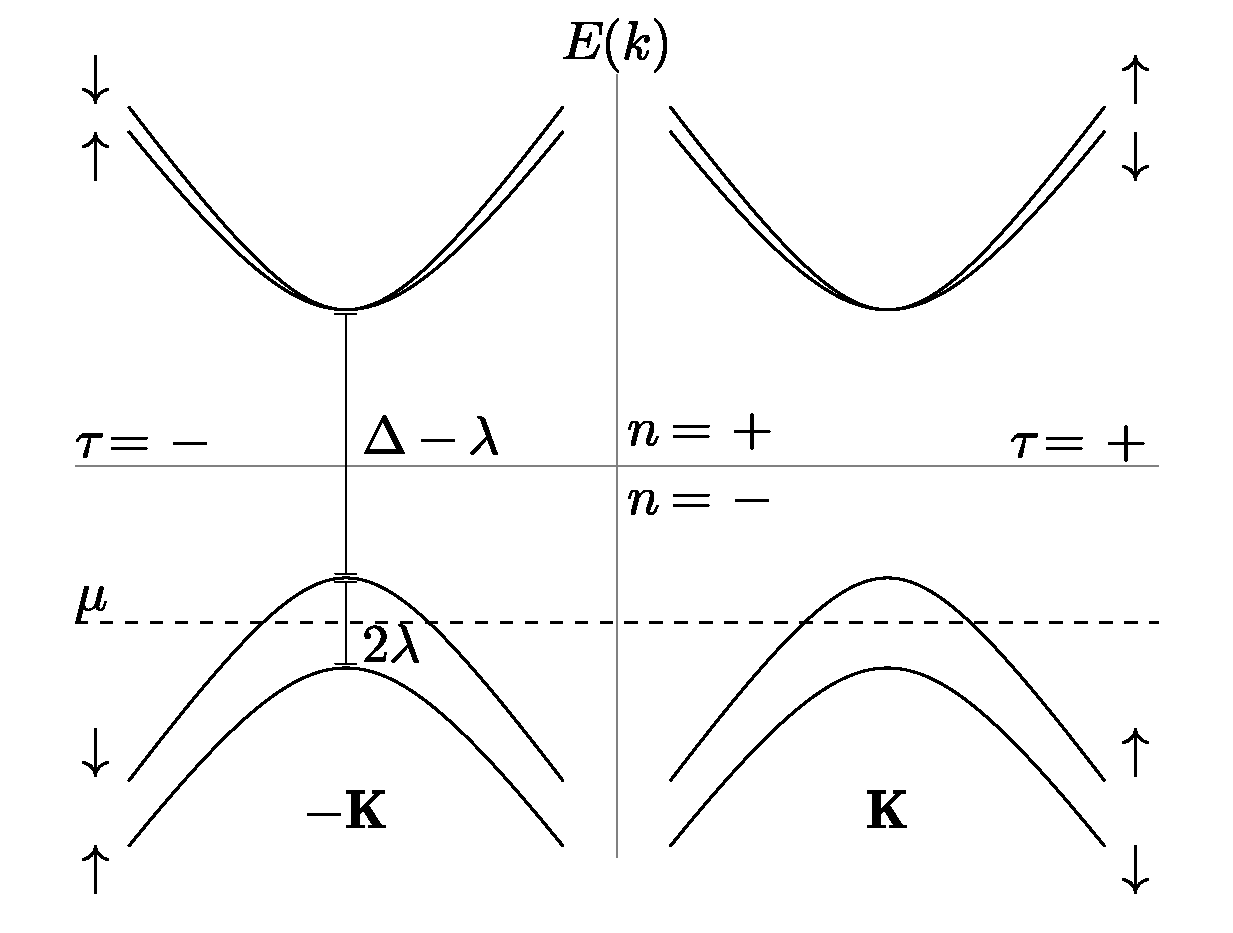
\includegraphics[width=\columnwidth]{figures/energy-bands}
\end{figure}
We focus on systems which have been doped
such that the chemical potential $μ$ lies in the upper valance bands.
Within each band, the Bloch basis eigenstates are written
in terms of the orbital states as elements on the Block sphere,
\begin{equation}
  \begin{aligned}
    \Ket{u_{τ {\s}}^n \of{k, ϕ}}
    = & \cos{\frac{\fnTheta{n}}{2}} \ketOrb{+}{\of{k, ϕ}} \\
    + e^{-i τ ϕ}
      & \sin{\frac{\fnTheta{n}}{2}} \ketOrb{-}{\of{k, ϕ}},
  \end{aligned}
\end{equation}
where $k_x + i τ k_y = k e^{i τ ϕ}$ and
\begin{equation}
  \tan{\frac{\fnTheta{n}}{2}}
  = \frac{a t τ k}{\dfrac{Δ}{2} - \fnEnergy{-n} \of{k}}
  = \frac{a t τ k}{\fnEnergy{n} \of{k} - \fnEnergy{-} \of{0}}.
\end{equation}
Note that the polar angle on the Bloch sphere
of the conduction and valence bands are related by
$\fnTheta{-} - \fnTheta{+} = τ π$.
The mapping of the energy band to the Bloch sphere,
parametrized by $\left( θ, ϕ \right)$,
encodes the topological character:
as one moves from the node out to infinity,
the states sweep either the northern or southern hemisphere
with a chirality determined by the Berry curvature.

  \section{Superconductivity}

We consider two approaches to realizing a superconducting state.
First, we assume a proximity induced state obtained by
layering a TMD on a suitable $s$-wave superconductor.
Second, we consider an intrinsic correlated phase arising
from density-density interactions.

In this section, we introduce the notation for the
Fock space creation and annihilation operators,
with $a^ν_{τ {\s}} \ofK$ corresponding to the tight-binding orbital states,
and $c^n_{τ {\s}} \ofK$ to the resulting eigenstates of the full Hamiltonian.

\subsection{Induced State}

A proximity $s$-wave superconductor will inject Cooper pairs
according to
\begin{equation}
  H^V
  = \sumK ∑_{ν, τ} \cc{Δ}_ν
    a^ν_{-τ ↓} \ofMK a^ν_{τ ↑} \ofK + \frac{ε}{2} + \hc
\end{equation}
The coupling constants $Δ_ν$ and the overall constant $ε$
will depend on the material interface.
Using the abbreviated notation
$c_{\vK α} = c^-_{τ {\s}} \ofK$,
with $α = ↑,↓$ for $τ = {\s} = ±$,
we project this into the upper-valance bands and obtain the Hamiltonian,
\begin{multline}
  \label{eq:induced}
  P_{τ = {\s}}^{n = -} \left( H^0 + H^V - μ N \right)
  = \sumK ∑_α ξ_{\vK} c_{\vK α}^† c_{\vK α} \\
    - \sumK \left( \cc{Δ}_{\vK} c_{-\vK ↓} c_{\vK ↑}
    + Δ_{\vK} c_{\vK ↑}^† c_{-\vK ↓}^† \right)
    + ε,
\end{multline}
where $ξ_{\vK} = E_{+ ↑}^- \of{\abs{\vK}} - μ$ and
\begin{equation}
  Δ_{\vK}
  = \frac{1}{2} \left( Δ_+ + Δ_- \right)
    +
    \frac{1}{2} \left( Δ_+ - Δ_- \right)
    \cos{θ_{\vK}},
\end{equation}
with $θ_{\vK} = θ_{+↑}^- \of{\abs{\vK}}$.
This form is identical to the standard BCS Hamiltonian with
an effective spin index $α$.
However, the spin state of the cooper pair is an equal superposition
of the singlet and the $m = 0$ component of spin triplet.
The corresponding energies,
$λ_{\vK} = ± \sqrt{ξ_{\vK}^2 + Δ_{\vK}^2}$,
and quasiparticle eigenstates,
$b_{\vK α}
= α \cos{β_{\vK}} c_{\vK α} + \sin{β_{\vK}} c_{-\vK, -α}^†$,
follow immediately.
Note that $Δ_{\vK}$ is a constant and independent of $\vK$
for $Δ_+ = Δ_-$.
Even when $Δ_+$ and $Δ_-$ are different,
the constant term is dominant.

We will return to this result after discussing the
intrinsic case as we will show the dominant channel mimics this form.

\subsection{Intrinsic Phase}

For a local attractive density-density interaction
(e.g.\ one mediated by phonons), the potential is
$V ⋍ \frac{1}{2} ∑_{\vR, \vR'} v_{\vR \vR'}
\normalorder{n_{\vR} n_{\vR'}}$,
with $v_{\vR \vR'} = v_0 δ_{\vR \vR'}$
and $n_{\vR}$ the total Wannier electron density at lattice vector $\vR$.
Projecting to the states near the chemical potential gives
\begin{multline}
  \label{eq:channels}
  P_{τ = {\s}}^{n = -} \left( H^V \right)
  = \sumKK v \of{\vK' - \vK} \\
  × \left(
    A_{\vK \vK'}^2 c_{\vK' ↑}^† c_{-\vK' ↑}^† c_{-\vK ↑} c_{\vK ↑}
  + A_{\vK' \vK}^2 c_{\vK' ↓}^† c_{-\vK' ↓}^† c_{-\vK ↓} c_{\vK ↓}
    \right. \\ + \left.
      2 \abs{A_{\vK \vK'}}^2
      c_{\vK' ↑}^† c_{-\vK' ↓}^† c_{-\vK ↓} c_{\vK ↑}
    \vphantom{2 \abs{V_{\vK \vK'}}^2} \right),
\end{multline}
where
\begin{equation}
  A_{\vK \vK'} =
    e^{i \left( ϕ_{\vK'} - ϕ_{\vK} \right)}
    \sin{\frac{θ_{\vK'}}{2}} \sin{\frac{θ_{\vK}}{2}}
    + \cos{\frac{θ_{\vK'}}{2}} \cos{\frac{θ_{\vK}}{2}}.
\end{equation}
The first two terms in \cref{eq:channels} lead to intravalley pairing,
and the third to intervalley pairing.
We analyze the possible states within mean field.
The order parameter is
\begin{equation}
  Δ_0 = v_0 \sumK \cc{g}_{\vK} \ev{c_{-\vK α'} c_{\vK α}},
\end{equation}
where the form of $g_{\vK}$ depends on the particular pairing channel.
The resulting Hamiltonian has the same form as the BCS Hamiltonian in
\cref{eq:induced}
with an effective $Δ_{\vK} = g_{\vK} · Δ_0$.
For intravalley channels, note that
$\ev{c_{-\vK α} c_{\vK α}} = - \ev{c_{\vK α} c_{-\vK α}}$,
thus relabeling $\vK → -\vK$ in the sum gives $Δ_0 = 0$ %
\footnote{%
  For complex interactions where
  $v \of{\vK} ≠ v \of{- \vK}$,
  the intravalley order parameters will in general be nonzero.
}.
The intervalley pairing has three symmetry channels,
with the couplings given by
$g_{\vK} = \sqrt{2}$,
$g_{\vK} = \sqrt{2} \cos{θ_{\vK}}$,
and $g_{\vK} = \sqrt{2} \sin{θ_{\vK}}$.
Of the three,
the constant valued channel is dominant %
\footnote{%
  For example, using the values for \ce{WSe2},
  $\sin^2 {θ_{\vK}} = 0.44$ and $\cos^2 {θ_{\vK}} = 0.56$
  at the chemical potential.
}.

This is to be expected as the local density-density interaction
leads to the largest pairing for electrons of opposite spins.
Since the intravalley processes have the same spin,
they are disfavored as compared to the intervalley pairing.
This result further suggests that intravalley pairing requires
odd parity couplings which may arise from spin exchange interactions.
Thus, the key features of the intrinsic superconducting state
are identical to the proximally induced case, and we restrict further
analysis to that case.
We now turn to the question of pair breaking phenomena
induced either by optical or magnetic fields.

  %\section{Optical Excitations}

\textit{Opto-electronic coupling:} The parent compound displays valley selectivity.
One circular polarization couples to one valley,
and the opposite to the other.
We investigate the extent to which this property
is inherited by the superconducting phase.
Note that one does not expect any dipolar coupling
since the orbitals involved have the same parity.
The optical excitations arise from the Berry curvature,
which acts as an effective angular momentum.
The electromagnetic potential $\vc{A}$,
with polarization vector $\vc{ϵ}$,
is introduced using minimal coupling,
\begin{equation}
  H_{τ σ}^{ν ν'} \ofK
  → H_{τ σ}^{ν ν'} \of{\vK + e \vc{A}},
\end{equation}
where, in the dipole approximation,
$\vc{A} = 2 \re{\vc{ϵ} A_0 e^{- i ω t}}$.
This yields a perturbed Hamiltonian
$H → H + H^A$, where
$H^A = H' e^{- i ω t} + H'^† e^{i ω t}$,
\begin{multline}
  H'
  = \sumK ∑_{τ, σ}
    H'_τ
    {a^v_{τ σ}}^† \ofK
    a^c_{τ σ} \ofK \\
  - \sumK ∑_{τ, σ}
    H'_{-τ}
    {a^c_{τ σ}}^† \ofK
    a^v_{τ σ} \ofK,
\end{multline}
and
\begin{equation}
  H'_τ
  = a t e A_0
    \left( τ \vc{\hat{x}} + i \vc{\hat{y}} \right)
    · \vc{ϵ}.
\end{equation}
The transition rate is proportional to the modulus-squared
of the optical matrix elements,
$\vc{P}_{τ σ}^{n n'} \ofK$,
defined by
\begin{multline}
  H^A
  = ∑_{\substack{\vK, τ, σ \\ n, n'}}
    \frac{e A_0}{m_0}
    \vc{ϵ} · \vc{P}_{τ σ}^{n n'} \ofK
    {c_{τ σ}^n}^† \ofK
    c_{τ σ}^{n'} \ofK.
\end{multline}

For circularly polarized light, in the absence of superconductivity,
$\vc{ϵ}_± = \left( \vc{\hat{x}} ± i \vc{\hat{y}} \right) / \sqrt{2}$ and
\begin{equation}
  \label{eq:optical}
  \vc{ϵ}_± · \vc{P}_{τ σ}^{+ -} \of{\vK}
  = ∓ τ \sqrt{2} a t m_0
    e^{± i ϕ}
    \sin^2 {\frac{\fnTheta{∓ τ}}{2}}.
\end{equation}
Since $\fnTheta{-} - \fnTheta{+} = τ π$,
switching either the valley or polarization transforms
$\sin → \cos$ in \cref{eq:optical},
leading to the valley selectivity in optical excitations.
For excitations above the BCS state,
the transition rate is given by \cref{eq:optical}
multiplied by a coherence factor $\sin^2 {β_{\vK}}$.
Thus, the superconducting phase exhibits
the same strong optical-valley coupling
for circularly polarized light.
This is shown in \cref{fig:optical.transitions}.
\begin{figure}
  \caption{%
    Optical transition rate matrix elements
    $\left| P_± \right|
    = \left(c / ℏ \right) \left| \vc{ϵ_±} · P_+^{+ -} \sin {β} \right|$
    for \ce{MoSe2}, \ce{WS2}, and \ce{WSe2}.
  }\label{fig:optical.transitions}
  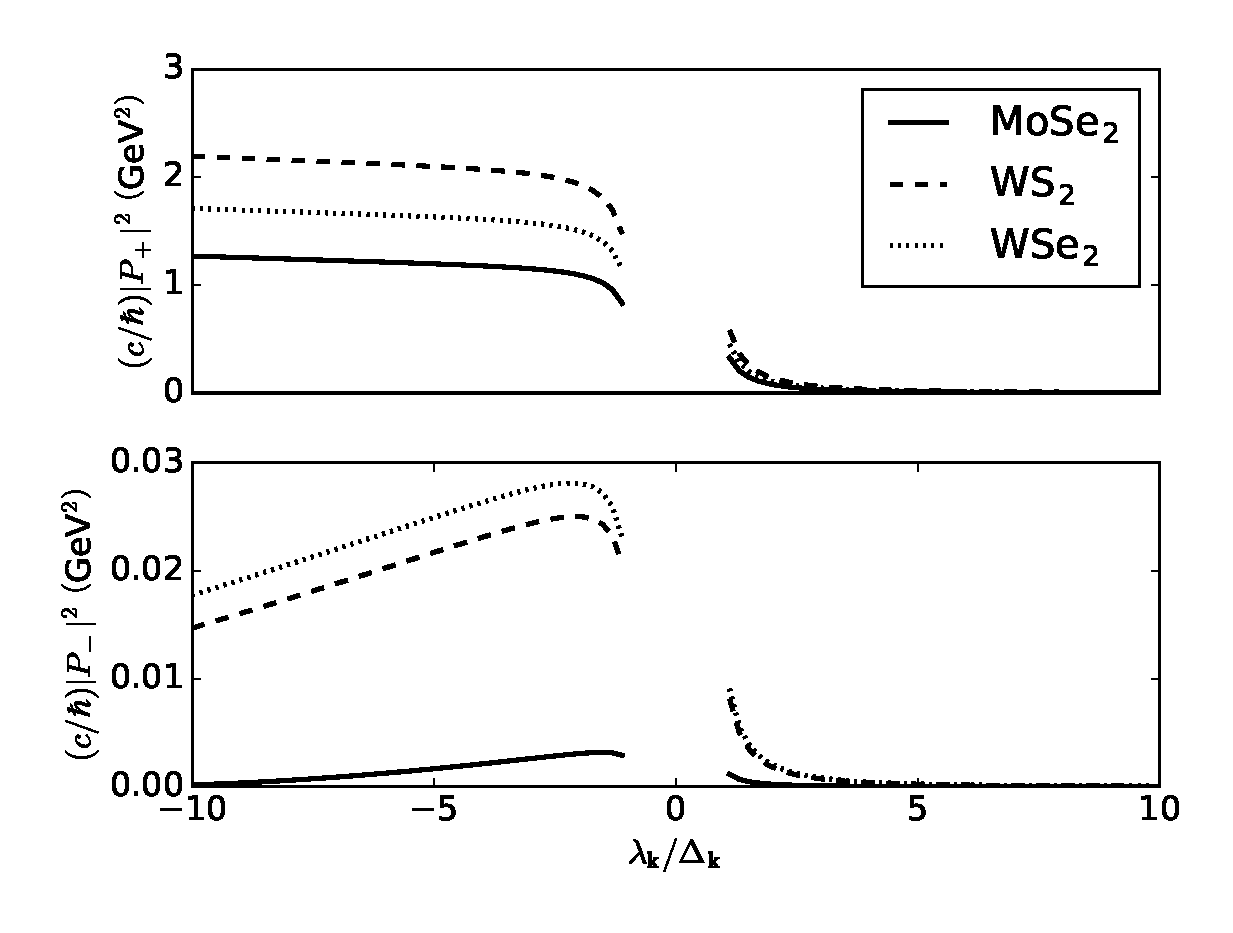
\includegraphics[width=\columnwidth]{figures/optical-transitions}
\end{figure}

For a given valley, a given polarization of light couples more strongly
than the other, as is evident comparing $\abs{P_+}$ to $\abs{P_-}$.
The suppression of the matrix elements above the chemical potential
reflects the fact that the BCS states include the Fermi distribution.
As such, the matrix element is still finite,
but is multiplied by a vanishing occupation probability.
The key new feature is the suppression of the valley contrast
as one approaches the chemical potential.
Nevertheless, for energies where the Cooper pair
is broken into quasiparticles well above the gap,
the superconducting state inherits the
valley selective phenomena of the parent compound.

  \section{Berry curvature}

The Berry curvature in the non-interacting crystal
for left and right circularly polarized
($\vc{ϵ}_±$) optical excitations for a given $\vK$
is $± 2 Ω_{+ ↑}^+ \of{k}$, where
\begin{subequations}
  \begin{align}
    Ω_{τ {\s}}^n \of{k}
    & = \vc{\hat{z}} · \vc{Ω}_{τ {\s}}^n \ofK, \\
    & = - n τ
        \left[ \frac{1}{2 k} \pderiv{}{k} \fnTheta{n} \right]
        \sin{\fnTheta{n}}, \\
    & = - n τ
        \frac{2 {\left( a t \right)}^2 \left( Δ - λ τ {\s} \right)}
        {{\left[{\left( 2 a t k \right)}^2
      + {\left( Δ - λ τ {\s} \right)}^2 \right]}^{3/2}}.
  \end{align}
\end{subequations}

The BCS ground state %
\footnote{%
  Note that the full ground state
  also contains the two lower filled bands,
  but those contribute zero net Berry curvature and may be ignored
  in this section and the next.}
is
\begin{subequations}
  \begin{align}
    \Ket{Ω}
    & = ∏_{\vK} \csc{β_{\vK}} γ_{\vK ↑} γ_{-\vK ↓} \Ket{0}, \\
    & = ∏_{\vK} \left( \cos{β_{\vK}} - \sin{β_{\vK}}
        c_{\vK ↑}^† c_{-\vK ↓}^† \right) \Ket{0}.
  \end{align}
\end{subequations}
This superconducting state is built up
from the quasiparticle eigenstates,
$\Ket{\vK}
= \csc{β_{\vK}} γ_{\vK ↑} γ_{-\vK ↓} \Ket{0}$,
of the $\vK$-dependent Hamiltonian
$λ_{\vK} \left( γ_{\vK ↑}^† γ_{\vK ↑}
+ γ_{-\vK ↓}^† γ_{-\vK ↓} \right)$.
The $z$-component of the Berry curvature of
the correlated state is zero,
\begin{equation}
  \vc{\hat{z}} · i ∇_{\vK} ⨯
  \Braket{\vK | ∇_{\vK} | \vK}
  = Ω_{+ ↑}^- \of{k} + Ω_{- ↓}^- \of{-k} = 0.
\end{equation}
A single optically excited state in the left valley
for a given $\vK$ is
${c_{+ ↑}^+}^† \ofK c_{+ ↑}^- \Ket{\vK}$,
which has a Berry curvature
$+2 \sin^6 {β_{\vK}} Ω_{+ ↑}^+ \of{k}$.
The corresponding excitation in the right valley
has a Berry curvature of the same magnitude but opposite sign.

  \section{Effect of in-plane magnetic field}

We briefly discuss the pair breaking effects
of an in-plane magnetic field and non-magnetic disorder.
(The details are presented elsewhere %
\footnote{%
  Junhua Zhang, Evan Sosenko, and Vivek Aji, in preparation.}.)

The superconducting state exhibits an anomalous magnetic response
due to the large spin-orbit interaction and spin splitting $λ$.
Unlike conventional superconductors,
where a uniform magnetic field
leads to pair breaking from spin paramagnetism,
here the Zeeman coupling from an in-plane magnetic field
in the clean system modifies the spin structure
of the Cooper pair, and parametrically suppresses $T_{c}$
in a mild way.
Modification of the effective coupling, rather than pair breaking,
causes this phenomena.
While, in compliance with Anderson's theorem,
the lack of pair breaking for nonmagnetic impurities is recovered at zero field
(since time reversal symmetry is preserved),
the transition is indeed suppressed by a pair-breaking effect
from the combination of the magnetic field and scalar impurities.

The pair breaking effect is characterized by the parameter
$δ_c
= τ_0^{-1} {\left( μ_B H_c^∥ / λ \right)}^2$,
where $μ_B$ is the Bohr magneton and $τ_0^{-1}$ is
the collision rate resulting from the scalar disorder potential.
Note that for a clean system, where $\tau_{0} \rightarrow \infty$,
we recover the result that there is no pair breaking.
%
Assuming a continuous phase transition induced by the magnetic field,
the pair-breaking equation at temperature $T$ is
\begin{equation}
  \log{\of{\frac{T_c'}{T}}}
  = ψ \of{\frac{1}{2} + \frac{δ_c}{2 π k_B T}}
  - ψ \of{\frac{1}{2}},
\end{equation}
where $ψ \of{z}$ is the digamma function,
$T_c'$ is the transition temperature
in the clean system
(mildly reduced by the in-plane field),
and $k_B$ is the Boltzmann constant.
This equation determines the upper critical field
$H_c^∥ \of{T}$ as a function of temperature.
Clearly, the upper critical field is greatly enhanced
by the large spin-orbit interaction.
At zero temperature, an approximate expression for the upper
critical field can be obtained as
\begin{equation}
  μ_B H_c^∥ \of{0}
  = λ \sqrt{2 π k_B T_c' τ_0 e^{ψ \of{1 / 2}}}.
\end{equation}

  \section{Conclusions}

In this letter, we report on the nature of the superconducting state
of hole-doped TMDs.
Remarkably, the correlated state inherits
the valley contrasting phenomena of the parent state.
While the magnitude is smaller, pair breaking produces quasiparticles
that have the same Berry curvature, and hence the same anomalous velocity.
Thus, one predicts an anomalous Hall response similar to
the one observed in \ce{MoSe2}.
Further consequences of the phenomena will be explored elsewhere.

Spin-valley locking leads to large critical magnetic fields.
A similar phenomena was recently reported in heavily hole-doped
(beyond the spin-split gap) \ce{NbSe2}.
In the new regime, where only one band per valley intersects
the chemical potential, no pair breaking occurs
for in-plane fields unless disorder is present.

While systematic synthesis and characterization of hole-doped systems
is still in its early stages, the fact that other two-dimensional compounds
and their bulk counterparts are known to be superconducting
provides impetus to explore the novel phenomena described here.

  \paragraph{Acknowledgments}

The software developed and used for this work
and the included figures is available freely online
\footnote{%
  Related software and source code at \\
  \url{https://evansosenko.com/dichalcogenides/}
}.
We thank Michael Phillips for useful discussions.
We acknowledge the support of Army Research Office through the grant
ARO W911NF1510079.


  % Must keep on single line or latexpand will fail.
  \bibliography{components/references/dichalcogenides,components/references/software,components/references/superconductivity}
\end{document}
